\subsubsection{Motivations}

Whilst the relatively simple mathematical constructs of the ML models, that are applied together with the physics-inspired structure descriptors, provide us with high degrees of interpretability to deepen our fundamental understanding on the chemistry-structure-property relationships of materials, which have been reviewed with many examples in \cref{sec:supervised_ML} and \ref{sec:unsupervised_ML}, they also imposed significant constraints for broadening the scopes, as well as increasing the levels of physical complexities, of the problems to which these models can be applied. There are a few fundamental reasons behind these limitations. 

Firstly, physics-inspired structure descriptors handle symmetries through a `baked-in' manner via the extensive use of tensor decomposition techniques, which,  as seen in \cref{sec:physics_informed_representation}, are typically achieved through the computations of the CG coefficients whose values are generally fixed. Whilst such an approach is pragmatic for preserving the invariance and equivariance of the structural features, they do not enlarge the space for \emph{optimising} the representations. The descriptors are thus \emph{fixed} in a sense that they are chosen and optimised for one class of material system (\emph{e.g.} bulk inorganic solids) and a specific learning task (being either unsupervised or supervised for a chosen target property), which may not work well for another system and/or learning task. This is easy to understand, as descriptors constructed in this way are pre-fixed into a feature space to highlight a subset of dominating features towards the learning target, which may not be transferable to another learning task. In another word, such a fixed descriptor approach is weak in terms of generalisability and adaptabilities, often capped by the sparsity of the high-dimensional space\cite{beyer1999nearest} and the size of the kernel matrix that can be handled numerically. 

On the other hand, in neural-network-based DL approaches, the latent representations of materials and the model parameters can be dynamically and jointly optimised with respect to the prediction targets and the additional exposures to new training data (the  process that has been commonly referred to as  \textit{fine-tuning}\cite{radova2025fine,bertani2025atomic,grandel2026parameter}), due to the flexibility provided by the large hyperparameter space ($\sim10^{6}$) over which the models can be optimised with the use of huge set of training data ($\sim10^{4}-10^{6}$).  This opens the opportunities to train universal foundational models that can be generally applied across materials system(s)\cite{batatia2023foundation,feng2025universal,wood2025family} for a wide variety of downstream tasks\cite{martin2025general,zhong2025machine,elena2025machine,ho2026equivariant} with the opportunity of solving classical theoretical problems with new tools from AI,\cite{goonnheimer2025beyond} making the DFT-level universality and accuracy for atomistic materials modelling achievable at the cost of forcefields to significantly expedite the process of materials discoveries.

Secondly, most structural descriptors were constructed with strong prior assumption in locality through the usages of, the cut-off distance $r_c$ that predefines the spatial range of interactions, and the body order $\nu$ that predefines the maximal number of neighbours that a given central atom can `see'. It is clear that a wide range of physical interactions, including electrostatics, non-covalent interactions,\cite{grisafi2021multi} charged defects,\cite{freysoldt2011electrostatic} anharmonic vibrations,\cite{darby2022compressing,yang2021altas} and conformational changes in molecules,\cite{frank2022so3krates} are long-ranged and/or entailing the cooperative interactions across many atoms. As such, a pragmatic approach would be to learn the effective cut-off and body-order from the data itself. Such a mechanism is apparently lacking in the paradigm of descriptor-based ML at this stage.

Lastly, the complexity involved in mapping the atomistic structure to its descriptor $\bm{R}\to\boldsymbol{\chi}$ implies that the reverse mapping from $\boldsymbol{\chi}$ back to a plausible structure $\bm{R}$, an endeavour that is needed for the inverse generative designs of new materials, will be almost impossible with simple ML-based approaches.

In these regards, the adaptation of the DL paradigm  have provided new opportunities to enhance our capabilities in data-driven  atomistic molecular and materials modelling. Increasing interests and development efforts that are devoted to the development of DL techniques can be seen over the past two decades.\cite{behler2021four} Rather than providing a full historical account, in the present and the next section, we shall provide an account on the current state-of-arts DL architectures for materials modelling, focusing on the key design concepts that enable us in building data-efficient, stable and robust models, respecting the fundamental physical principles. A particular focus will be on how equivariance is enforced in the modern graph neural networks (GNNs),\cite{duval2023hitchhiker} that are subtlety different from the construction of equivariant structural descriptors for atomistic ML, as discussed in \cref{sec:physics_informed_representation}.

\subsubsection{Preliminaries on the Principles behind Neural Networks}

As discussed above, kernel-based ML heavily leverages on the designs and engineering of feature vectors and kernels to account for nonlinearity in the data. In contrast, NNs from the DL paradigm take a distinctively different approach, which, in this section, we shall provide the readers with some baseline understandings on the principles behind NNs to facilitate the subsequent discussions on the modern equivariant NN architectures for atomistic molecular and materials modellings. 

\begin{figure}[tbh]
    \centering
    \includegraphics[width=0.8\linewidth]{simple_nn_illustrate.pdf}
    \caption{Illustrations on the conceptual understandings on the working principles behind neural networks and their relevance to pairwise interactions in atomistic systems. (a) A simple network that maps an input $x$ to an output $y$ with three nodes $h_i$ in the middle layer. Each node is modelled by a ReLU-type activation function, the output of which will be weighted by $w_i$, before the output of all three nodes are added together to generate the output. (b) Using simple network to surrogate a smooth function of the type of a double potential well can be seen as fitting piecewise linear functions with different gradients ($k$) that are joined at multiple `hinge points' $x_h$, where $k$ and $x_h$ are to be optimised. With sufficient number of hyperparameters, this surrogate model will be able to reproduce the nonlinear target function as shown in (c). (d) An schematic illustration of a simple, densely interconnected, deep neural networks with 4 input nodes (blue circles), 4 hidden layers (open circles)  and 1 output node (green circle). (e) Analogous example on how simple neural network is trained to understand the connectivity in a molecule, in which the training starts by putting equal weight (leftmost) on all pairs of atoms in the structure, and as training progress, the weights essentially become dominated by the connections that correspond to the existence of interatomic covalent bonds (rightmost). }
    \label{fig:simple_nn_illustrate}
\end{figure}


In its simplest form, NN tries to map simple input  with zero or minimum feature engineering, into highly non-linear functions (or features) by passing the data through multiple \textit{interconnected neurons}, each carries out some simple (often linear) mathematical transformations,\cite{prince2023understanding} that collectively allows the model to learn complex relationships between the input and output. As an example, \cref{fig:simple_nn_illustrate}(a) demonstrates the construct of a simple NN that contains a single input node that maps a simple input $x\in\mathbb{R}$ (which for simplicity, we shall assume $x\sim \mbox{Uniform}([0,1])$) into a single output node with the corresponding output of $y$. The middle layer contains 3 hidden units, each of which takes the form of a \emph{rectified linear unit (ReLU)} or otherwise known as the \emph{activation function}, that transforms the input with the following function:
\begin{equation}
    \label{eq:ReLU}
    h_i(x)=\max(0,k_ix+b_i).
\end{equation}
Suppose $k_i>0$, then it is easy to see that each neuron will act on the input and map $\forall x>x_h=-b_i/k_i$ (which we shall call $x_h$ the hinge point) to a linear segment $k_ix+b_i$. The output from each hidden unit is then subsequently weighted by a weighting parameter $w_i$ before the outcomes from all three hidden units are added together for the final outcome, \emph{i.e.} 
\begin{equation}
    \label{eq:NN_additivitiy}
    y=\sum_i w_ih_i(x).
\end{equation}


As shown in \cref{fig:simple_nn_illustrate}(b), this approach effectively breaks down a smooth non-linear function into a piecewise linear one that is joined at multiple hinge points. It is therefore easy to envisage, that by increasing the number of hidden layers and nodes in each layers to form densely connected deep NN [\cref{fig:simple_nn_illustrate}(d)], the model will have the potential to optimise a large set of hyperparameters $\{\bm{k},\bm{b},\bm{w}\}$ that allows the target functions to be accurately regressed in finer details as more piecewise linear functions were used in the fitting    [\cref{fig:simple_nn_illustrate}(c)]. This provides us with an intuitive understanding on how, by stacking multiple simple mathematical transformations in layers, NN is able to learn the complex nonlinear relationships in the the underlying data. 

Most importantly, the usage of simple activation functions $h_i(x)$ enable its derivatives to be efficiently computed analytically, where the total functional derivative of the output with respect to the input  ($\partial y/\partial x$) can now be computed through the \emph{back propagation} algorithm, enabling the gradient-based minimisations of the loss function for model training. This is typically combined with \emph{stochastic gradient descents},\cite{prince2023understanding} especially when training NN with large datasets, that introduces randomness in the gradient-descent process by using different batches of the training samples at each step, allowing the optimisation algorithm to more effectively jump out from the local minima and cross the saddle points in the landscape of the loss function.  This provides significant numerical advantages compared to, for example, the optimisations of parameters in traditional atom-atom forcefields [\cref{sect:empirical_forcefield}], in which the different forcefield terms can become highly coupled, leading to trench-shaped loss function landscape that does not lead to an optimum solution. Problems like this often require tailored designed training sets that allow different terms in the forcefields to be individually fitted, or imposing  constraints building upon prior knowledges, to regularise the overall fitting process, which can be mitigated by adapting the DL approach for developing NN potentials for atomistic modellings.

In a more physical context, when the NN is used to train an energy model that outputs the system energy $E$ with respect to the input, that is usually  the atomic positions $\bm{R}$, the back-propagation algorithm enables us to compute and learn the atomic forces via $F=-\partial E/\partial \bm{R}$ that is particularly useful for dynamic simulations. This leads to the so-called \emph{energy conserving} energy model, as opposed to those \emph{non-conserving} models in which the atomic forces are trained with a separate model from the system energies.
 
Training the NN, in which the weight parameters are optimised, reflecting how strongly one neuron influences another, can be understood by drawing parallel examples on how chemical bond emerge in atomistic systems heuristically [\cref{fig:simple_nn_illustrate}(e)]. In this analogous example, one can consider the initial state of the system being one that contains a collection of atoms, in which all pairs of atoms interact with equal strength. In terms of NN training, this corresponds to initialising the NN with equal weight across all connected neuron pairs. As time continues, electrons in space will `feel' the field established by the nuclei and gradually redistribute towards regions that minimise the total system energy, during which chemical bonds will appear between selected pairs of atoms in the system where the covalent interactions should exist. This is the same process in which weights are optimised throughout the NN, by putting higher weights on neuron interactions (or information passing pathways) that are expected to contribute most significantly in transforming the input data to the corresponding outputs.  Such concepts underpin the designs and implementations of modern equivariant GNNs for atomistic modellings, which,  we shall provide a brief account on the key features of equivariant GNNs in the following section.

\subsubsection{Equivariant Graph Neural Networks}

In mathematical chemistry, molecules have seen a long tradition in being modelled as graph-type objects, dating back to 1870s.\cite{cayley1874lvii} It is therefore, unsurprising to see chemistry being the early adaptor of the GNN model.\cite{duvenaud2015convolutional} In 2017, \citet{gilmer2017neural} further proposed the message-passing GNNs (MPNNs) for molecules, which has since became one of the most popular and mainstream DL architectures for atomistic molecular and materials modellings. Most importantly, the incorporation of symmetries through extensive use of group and representation theory in the model architecture, as opposing from earlier NN models\cite{behler2021four} which heavily reply on the use of handcrafted descriptors,  has become an important inductive bias in the model design to enhance the models' data efficiency and ability of extrapolations.\cite{fu2022forces,frank2022so3krates} In terms of fundamental architectural designs behind MPNNs, the hitchhiker's guide written by \citet{duval2023hitchhiker} has provided a good comprehensive pedagogical reference to understand the fundamental mathematical principles behind the invariant and equivariant GNNs. On a more application-oriented focus, \citet{ reiser2022graph} reviewed the development of GNNs for molecular and materials science up to 2022. 

To be inline with our previous discussions on physics-inspired density-field structure descriptors in \cref{sec:physics_informed_representation}, in this section,  we shall provide a more focused and concise account of the key concepts behind, and general approaches in incorporating the invariant and/or equivariant symmetry constraints, as well as accounting for many-body orders, in modern message-passing GNNs, that are different from the descriptor-based approaches. As a more concrete example, we will review how the MACE\cite{batatia2022mace} model architecture has up-taken a more principled approach that combines equivariant atom-centred interatomic potential\cite{drautz2019atomic} and MPNNs, that allows features up to any arbitrary order of $\nu$ to be learned with MPNN. We further assume that the primary focus here is the application of GNN for developing energy models, although equivariant GNNs see a wide range of scenarios in which it may be applied, for instances, as the backbones for generative models, to be discussed in \cref{sec:generative_AI}.

\begin{figure}[tbh]
    \centering
    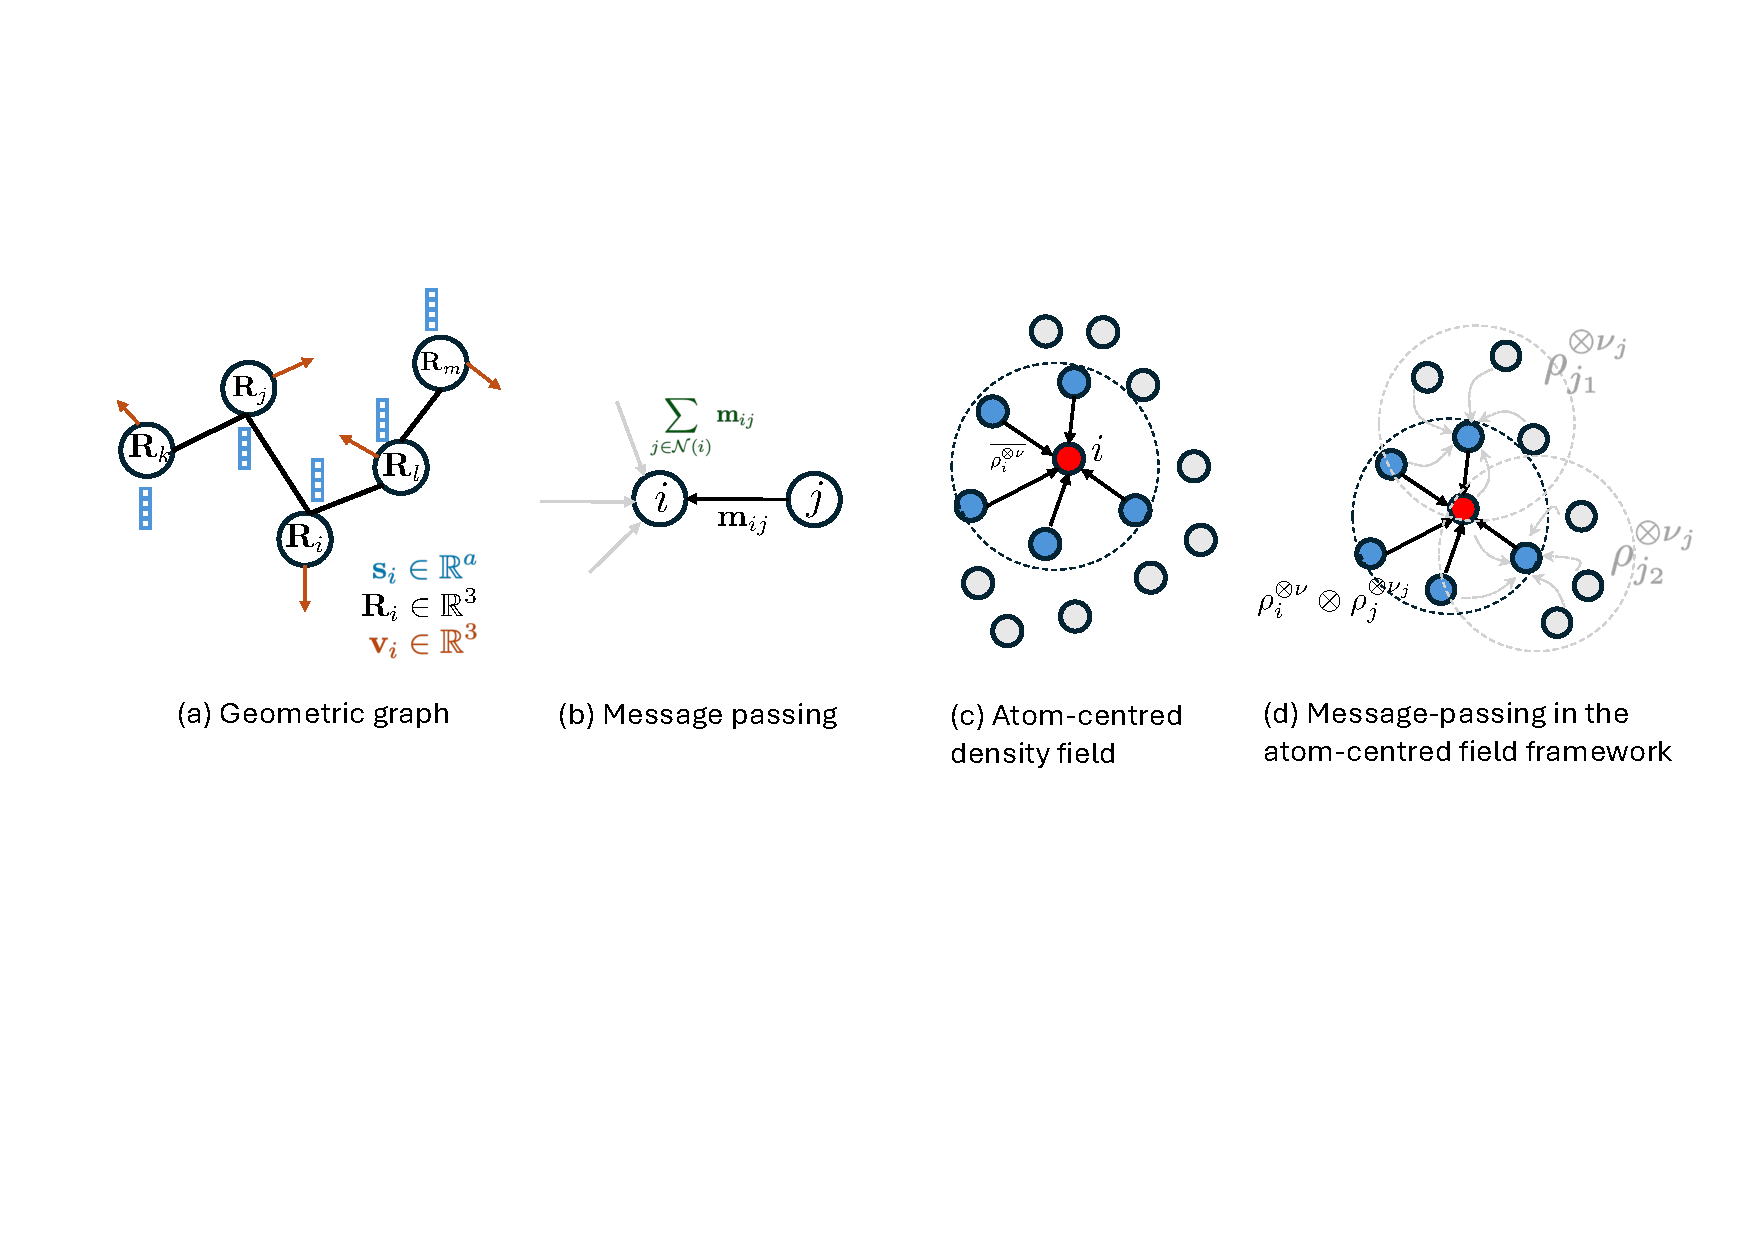
\includegraphics[width=\linewidth]{massage-passing.pdf}
    \caption{Core concepts behind message-passing graph neural networks. (a) Atomistic structure can be modelled as geometric graph in 3D Euclidean space\cite{duval2023hitchhiker} consists of nodes that represent atoms that are connected by edges, which represents bondings between atoms. Each node is associated with a set of mathematical attributes such as $\bm{s}_i$ which carriers chemical information constructed through N.N. embedding and transforms invariantly, and the Cartesian coordinates $\bm{R}_i$ and velocity (or forces) $\bm{v}_i$ that transform equivariantly under translation and rotation. (b) Message passing operation, where each central node $i$ learns its latent representation by receiving and aggregating the messages $\bm{m}_{ij}$ from all of its local neighbours $j\in\mathcal{N}(i)$. The way that message-passing formalism builds latent representations can be understood from the perspectives of atom-centred density field representations in which (c) in its original construct, the central atom $i$ sees the `bare' densities from each one of its neighbouring atoms $j$ within a pre-defined cut-off, whereas in the message-passing scheme (d) the centre atom interacts with the `dress' densities from the neighbours, whereby  each neighbour atom $j$ also aggregates information from its own surrounding neighbours through tensor product operation $\rho_{j_k}^{\otimes\nu_j}$ before they are interacting with the central atom $i$ through the operation of $\rho_i^{\otimes\nu}\otimes\rho_{j_k}^{\otimes\nu_j}$.
     }
    \label{fig:massage-passing}
\end{figure}

The starting point of GNN is to treat an atomistic structure of molecule/material as graphs in which atoms that are connected together by chemical bonds can be treated as \emph{nodes} that are connected by \emph{edges} in the graph representation. Two nodes are said to be connected if there exists an edge connecting the two nodes, the information of which is generally encapsulated in the connectivity matrix $\bm{A}$ that takes a matrix element of value 1 for two connected nodes and 0 otherwise. Practically, the connectivity between nodes are generally determined using the `neighbourhood' approach based on a pre-defined cut-off radius  $r_c$,  as  similar to that of \cref{eq:atom_env_density_field}, so the definition of an \emph{edge} is not necessarily confined to the existence of a covalent/ionic bond between a pair of atoms, but more align with the physical concept of `field' within the 3D space.  Furthermore, the graph object that is constructed for atomistic modelling is not a simple graph but is what generally referred to as the \emph{geometric graph} [\cref{fig:massage-passing}(a)], in which the nodes (optionally for edges as well) are further decorated with  a set of attributes that are either invariant (such as chemical identities $\bm{s}_i\in\mathbb{R}^a$ as a vectorial quantity constructed through embedding) or equivariant (such as the atomic coordinates $\bm{R}_i\in\mathbb{R}^3$ and atomic forces/velocities  $\bm{f}_i\in\mathbb{R}^3$) with respect to the translation and SO(3) rotations of the atomistic structures, in addition to the connectivity information $\bm{A}$.

With the establishment of the geometric graphs, MPNN further model the physical processes for formation of chemical bonds (or equivalently, the interactions among neighbouring atoms) as a mathematical operation of \emph{message passing} between connected nodes [\cref{fig:massage-passing}(b)]. In the message-passing paradigm, a given central node $i$ exchange message $\bm{m}_{ij}$ from every one of its connected neighbouring nodes $j$, in which we consider $\bm{m}_{ij}=f_{\boldsymbol{\varphi}}(i,j)$  as some parameterised NN function on node attributes, and the messages from all the neighbours are summed together in each round of message-passing, \emph{i.e.} $\sum_{j\in\mathcal{N}(i)}\bm{m}_{ij}$ to update the information on $i$. Conceptually, this can be considered as equivalent to constructing a two-body (one from the centre atom) atom-centred density field representation  [\cref{fig:massage-passing}(c)]. However, one must note that each neighbouring node $j$ is also connected to its own neighbours, and so on. In the simplest case, if we combine two message-passing layers, then we think of the information from the neighbours if a given atom $j$ are aggregated onto $j$ before its information is passing onto $i$, allowing $i$ to effectively `sees' atoms that are two connections away. In the atom-centred density-field framework, this effectively means that the central atom is not convoluting the `bare' density but a `dressed' one from its neighbouring environments [\cref{fig:massage-passing}(d)].\cite{nigam2022unified} In this regards, stacking multiple MP hidden layers in GNN essentially establishes a densely connected NN model [\cref{fig:simple_nn_illustrate}(a)] to mimic the interconnected atomistic systems in 3D space, whereas the \emph{receptive field} of a given central atom $i$, \emph{i.e.} how far away the chemical and structural information from distant atoms (measured in terms of number of edges), are passed onto $i$ in MPNN, can be controlled by the number of MP operations used in an MPNN.

Unlike the descriptor-based approach, where symmetry is baked into the descriptor designs, in MPNN, symmetry of the geometric graphs are preserved by carefully designing  mathematical transformations in the operations that construct, pass and update messages through diligently counting the allowed operations that preserve the invariant and/or equivariant geometry features up to some pre-defined maximum body order $\nu_{\max}$.\cite{duval2023hitchhiker} 



\begingroup % Start a group to localize the change
%\renewcommand{\arraystretch}{1.2}  
\LTcapwidth=\textwidth

\begin{longtable}{p{1.25cm}p{2.5cm}p{3cm}p{10.25cm}}
    \caption{A concise chronological list of major geometric/equivariant GNNs for molecular and materials modellings, which are predominantly developed for the application as MLFFs to accelerate PES samplings.}
    \label{tab:equivariant_GNNS}\\
    \hline\hline
     \textbf{\footnotesize{Year}}    & \textbf{\footnotesize{Model}}  & \textbf{\footnotesize{Domain}} &
      \textbf{Key features}\\
     \hline
     \endfirsthead
\caption*{Table \ref{tab:equivariant_GNNS} (Continued):A concise chronological list of major geometric/equivariant GNNs.  }\\\toprule
     \textbf{\footnotesize{Year}}    & \textbf{\footnotesize{Model}}  & \textbf{\footnotesize{Domain}} &
      \textbf{Key features}\\
     \hline
\endhead
\hline\hline
\endfoot
\hline\hline
\endlastfoot

\footnotesize{2017} &  
\footnotesize{SchNet\cite{schutt2017schnet}}&
\footnotesize{Molecules \& materials} & 
\footnotesize{Invariant features, up to 2-body order, convolution}\\

\footnotesize{2017} &  
\footnotesize{CGCNN\cite{xie2018crystal}}&
\footnotesize{Crystalline materials}& 
\footnotesize{Invariant features, up to 2-body order, convolution}\\

\footnotesize{2018} &
\footnotesize{TFN\cite{thomas2018tensor}} &
\footnotesize{Molecules} &
\footnotesize{SO(3) equivariant feature in spherical harmonic basis, up to 2-body order}\\

\footnotesize{2019} &
\footnotesize{PhysNet\cite{unke2019physnet}}&
\footnotesize{Molecules}&
\footnotesize{Invariant features, up to 2-body order with radial basis functions, convolution}\\

\footnotesize{2019} &
\footnotesize{DimeNet\cite{gasteiger2020directional}} &
\footnotesize{Molecules} &
\footnotesize{Invariant features, up to 3-body with radial and angular (spherical harmonic) basis functions, message-passing }\\

\footnotesize{2019} &
\footnotesize{Comorant\cite{anderson2019cormorant}} &
\footnotesize{Molecules} &
\footnotesize{Rotationally covariant features, up to 2-body order with spherical harmonics}\\

%footnotesize{2019} &
%\footnotesize{MEGNet\cite{}} &
%\footnotesize{} &
%\footnotesize{}\\

\footnotesize{2020} &
\footnotesize{DimeNet++\cite{gasteiger2020fast}} &
\footnotesize{Molecules} &
\footnotesize{Invariant features, up to 3-body, message-passing}\\

\footnotesize{2020} &
\footnotesize{MXMNet\cite{zhang2020molecular}} &
\footnotesize{Molecules} &
\footnotesize{Invariant features, up to 3-body, message-passing}\\

\footnotesize{2020} &
\footnotesize{LieConv\cite{finzi2020generalizing}} &
\footnotesize{Molecules} &
\footnotesize{Lie-group equivariant features, convolution}\\

\footnotesize{2020} &
\footnotesize{LieTransformer\cite{hutchinson2021lietransformer}} &
\footnotesize{Molecules} &
\footnotesize{Lie-group equivariant features, attention mechanism\cite{vaswani2017attention}}\\

\footnotesize{2020} &
\footnotesize{SE(3)-Transformer\cite{fuchs2020se}} &
\footnotesize{Molecules} &
\footnotesize{Equivariant SE(3) features, spherical harmonic basis functions, attention mechanism}\\

\footnotesize{2021} &
\footnotesize{SphereNet\cite{liu2022spherical}} &
\footnotesize{Molecules} &
\footnotesize{Invariant features, up to 4-body order, message-passing}\\

\footnotesize{2021} &
\footnotesize{GemNet\cite{gasteiger2021gemnet}} &
\footnotesize{Molecules \& materials \& catalysts} &
\footnotesize{Invariant features, up to 4-body order, directional message-passing}\\

\footnotesize{2021} &
\footnotesize{SEGNN\cite{brandstetter2021geometric}} &
\footnotesize{Molecules} &
\footnotesize{E(3) equivariant features, up to 2-body order in spherical harmonic basis, meassage-passing}\\

\footnotesize{2021} &
\footnotesize{EGNN\cite{satorras2021n}} &
\footnotesize{Molecules} &
\footnotesize{Invariant E($n$) features, up to 2-body order in Cartesian basis, message-passing}\\

\footnotesize{2021} &
\footnotesize{PaiNN\cite{schutt2021equivariant}} &
\footnotesize{Molecules} &
\footnotesize{Equivariant features, up to 3-body order in Cartesian basis, message-passing}\\

\footnotesize{2021} &
\footnotesize{NequIP\cite{batzner20223}} &
\footnotesize{Molecules \& materials} &
\footnotesize{E(3) equivariant features in spherical basis, up to 2-body order, convolution}\\

\footnotesize{2021} &
\footnotesize{SpookyNet\cite{unke2021spookynet}} &
\footnotesize{Molecules} &
\footnotesize{Invariant features, up to 2-body order, attention mechanism}\\

\footnotesize{2022} &
\footnotesize{TorchMD-Net\cite{tholke2022torchmd}} &
\footnotesize{Molecules} &
\footnotesize{Equivariant features in Cartesian basis, up to 2-body order, attention mechanism}\\

\footnotesize{2022} &
\footnotesize{EQGAT\cite{le2022equivariant}} &
\footnotesize{Molecules} &
\footnotesize{Equivariant features in Cartesian basis, up to 2-body order, message-passing and attention mechanism}\\

\footnotesize{2022} &
\footnotesize{ComENet\cite{wang2022comenet}} &
\footnotesize{Molecules} &
\footnotesize{Invariant features up to 4-body order, message-passing}\\

\footnotesize{2022} &
\footnotesize{So3krates\cite{frank2022so3krates}} &
\footnotesize{Molecules \& materials} &
\footnotesize{SO(3) equivariant features in spherical basis, up to 2-body order, message-passing with attention mechanism}\\

\footnotesize{2022} &
\footnotesize{Equiformer\cite{liao2022equiformer}} &
\footnotesize{Molecules \& catalysts} &
\footnotesize{SE(3) equivariant features in spherical basis, message-passing with attention mechanism}\\

\footnotesize{2022} &
\footnotesize{GemNet-OC\cite{gasteiger2022gemnet}} &
\footnotesize{Catalysis} &
\footnotesize{Invariant features up to 4-body order, message-passing}\\

\footnotesize{2022} &
\footnotesize{MACE\cite{batatia2022mace}} &
\footnotesize{Molecules \& materials} &
\footnotesize{Equivariant features in spherical and cluster-expansion basis, up to many-body-orders, message-passing}\\

\footnotesize{2022} &
\footnotesize{Allegro\cite{musaelian2023learning}} &
\footnotesize{Molecules \& materials} &
\footnotesize{Equivariant features in spherical basis, up to many-body-orders, message-passing}\\

\footnotesize{2022} &
\footnotesize{ClofNet\cite{du2022se}} &
\footnotesize{Molecules} &
\footnotesize{SE(3) equivariant features in Cartesian basis, message-passing}\\

\footnotesize{2023} &
\footnotesize{LEFTNet\cite{du2023new}} &
\footnotesize{Molecules} &
\footnotesize{Equivariant features in Cartesian basis, message-passing}\\

\footnotesize{2023} &
\footnotesize{ViSNet\cite{li2024long}} &
\footnotesize{Molecules} &
\footnotesize{Equivariant features in Cartesian basis, long-short-range message-passing}\\

\footnotesize{2023} &
\footnotesize{TensorNet\cite{simeon2023tensornet}} &
\footnotesize{Molecules} &
\footnotesize{Equivariant features in Cartesian basis, message-passing}\\

\footnotesize{2023} &
\footnotesize{eSCN\cite{passaro2023reducing}} &
\footnotesize{Materials \& catalysts} &
\footnotesize{Equivariant features in spherical harmonic basis, up to 2-body order, convolution}\\

\footnotesize{2023} &
\footnotesize{CHGNet\cite{deng2023chgnet}} &
\footnotesize{Materials} &
\footnotesize{Charge-aware equivariant features, convolution}\\

\footnotesize{2023} &
\footnotesize{M3GNet\cite{chen2022universal}} &
\footnotesize{Materials} &
\footnotesize{Equivariant features in Cartesian space, up to 3-body order, }\\

\footnotesize{2023} &
\footnotesize{EquiformerV2\cite{liao2024equiformerv2}} &
\footnotesize{Molecules \& materials \& catalysts} &
\footnotesize{SO(3) equivariant features, up to 2-body order, message-passing \& attention mechanism.}\\

\footnotesize{2024} &
\footnotesize{UMA\cite{wood2026family}} &
\footnotesize{Molecules \& materials \& catalysts} &
\footnotesize{Foundational model for atomistic modelling building on the eSCN equivariant model.}\\

\footnotesize{2024} &
\footnotesize{CACE\cite{cheng2024cartesian}} &
\footnotesize{Molecules \& materials}&
\footnotesize{Equivariant features in Cartesian basis as an alternative framework to MACE  to achieve higher-order correlations.}\\

\footnotesize{2025} &
\footnotesize{E$^2$GNN\cite{yang2025efficient}} &
\footnotesize{Molecules \& materials}&
\footnotesize{Equivariant features in Cartesian basis, message-passing}\\

\footnotesize{2025} &
\footnotesize{MGNN\cite{chang2025mgnn}} &
\footnotesize{Molecules \& materials}&
\footnotesize{Rotationally invariant features with moment-based representation learning, message-passing.}\\

\footnotesize{2026} &
\footnotesize{mMACE\cite{ho2026equivariant}}&
\footnotesize{Materials}&
\footnotesize{Building on the MACE framework to additionally take into account the equivariance of magnetic moments}
\end{longtable}

Most of the early implementations of MPNNs [\cref{tab:equivariant_GNNS}] have been focusing on constructing messages from scalar many-body features that transforms invariantly under symmetry operations, such as the chemical information, bond lengths (2-body), bond angles (3-body) and torsional angles (4-body), depending on the choice of $\nu_{\max}$. These messages are easy to construct, and closely resembles the use of internal coordinates [\cref{sec:coordinates_systems}] for constructing the atom-atom forcefields [\cref{sect:empirical_forcefield}]. For instance, using the node information on the geometric graph [\cref{fig:massage-passing}(a)] discussed above, a two-body invariant learnable message can be constructed by selecting tensor operations amongst the nodal and two-body features that will lead to scalar output, such as:\cite{duval2023hitchhiker}
\begin{equation}
    \label{eq:2-body-invariant-message}
    m_{ij}=f_{\boldsymbol{\varphi}_1}\left(\bm{s}_i,\Vert \bm{v}_i\Vert_2\right)+\sum_{j\in\mathcal{N}(i)}f_{\boldsymbol{\varphi}_2}(
    \bm{s}_i,
    \bm{s}_j,
    \Vert \bm{x}_{ij}\Vert_2,
    \Vert \bm{v}_j\Vert_2,
    \bm{x}_{ij}\cdot\bm{v}_i,
    \bm{x}_{ij}\cdot\bm{v}_j,
    \bm{v}_{i}\cdot\bm{v}_j),
\end{equation}
in which the interatomic vector $\bm{x}_{ij}=\bm{R}_i-\bm{R}_j$, whereas equivariant messages of a given order can be constructed by scaling the tensorial features that particular order with the scalar outputs from the learnable messages:
\begin{align}
\bm{m}_{ij}=f_{\boldsymbol{\varphi}_3}\left(\bm{s}_i,\Vert \bm{v}_i\Vert_2\right)\odot \bm{v}_i &+ \sum_{j\in\mathcal{N}(i)}f_{\boldsymbol{\varphi}_4}(
    \bm{s}_i,
    \bm{s}_j,
    \Vert \bm{x}_{ij}\Vert_2,
    \Vert \bm{v}_j\Vert_2,
    \bm{x}_{ij}\cdot\bm{v}_i,
    \bm{x}_{ij}\cdot\bm{v}_j,
    \bm{v}_{i}\cdot\bm{v}_j)\odot\bm{x}_{ij}\nonumber\\
    &+\sum_{j\in\mathcal{N}(i)}f_{\boldsymbol{\varphi}_5}(
    \bm{s}_i,
    \bm{s}_j,
    \Vert \bm{x}_{ij}\Vert_2,
    \Vert \bm{v}_j\Vert_2,
    \bm{x}_{ij}\cdot\bm{v}_i,
    \bm{x}_{ij}\cdot\bm{v}_j,
    \bm{v}_{i}\cdot\bm{v}_j)\odot\bm{v}_{ij}.
    \label{eq:2-body-equivariant-message}
\end{align}
It is thus easy to understand the inclusion of three-body features in the message would naturally include terms like the bond angles $\theta_{ijk}$, which may be constructed from dot-products $\bm{x}_{ij}\cdot\bm{x}_{ik}$, for an dihedral centred on $i$. Although this provides a physically intuitive way to understand how nodes can exchange information through the constructions of tensor products using geometric information that are native to computationalists on an practical basis, it does not leads to a pragmatic way to construct an arbitrary $\nu$-body invariant message as one needs to diligently keep track of all possible operations on different combinations of nodal features up to $\nu$ interacting nodes that can output a scalar feature.

The above problem is effectively overcome in the later variants of MPNNs [\cref{tab:equivariant_GNNS}], that uses the knowledge of tensor algebra, group and representation theory [\cref{sec:physics_informed_representation}] to construct and interact amongst tensorial quantities to construct equivariant messages from 0 up to some pre-defined maximal ranks. Drawing from our discussions on atom-centre density field representation, we can envisage that the primary goal here is to preserve and exchange angular information on the local chemical environments amongst the interacting pairs, triplets, and higher-order atomic clusters, which, as can be seen in \textbf{Box IV} that using the irreps of the SO(3) group in the spherical harmonic basis can provide the principled way to achieve our goal. 

In equivariant MPNN, this is typically started from the implementation of a feature mapping layer, that maps any vector properties, such as $\bm{x}_{ij}$ into the spherical harmonic basis up to the maximal rank of $\ell_{\max}$, giving a list of tensors $\vec{\bm{Y}}=[\vec{Y}^{(0)},\vec{Y}^{(1)},\ldots,\vec{Y}^{(\ell_{\max})}]$, where we only retain the angular information with $Y_\ell^m(\bm{x}_{ij}/\Vert \bm{x}_{ij}\Vert_2)\to Y_\ell^m$. Now the process of constructing the message, we can, in the message function $f_{\boldsymbol{\varphi}}$ to allow two list of tensors $\vec{\bm{T}}$ (which, in line with the definition, will encode the angular information between two bodies $i$ and $j$) and $\vec{\bm{S}}$ (which encodes two-body information between $i$ and $k$) to interact through tensor product, similar to the process of constructing $\rho^{\otimes 2}$ in SOAP (\cref{fig:soap_invariant_tensor_prod}), but instead of retrieving only the invariant component of the tensor products, we can retrieve tensors of all other allowed ranks as well. 


\begin{figure}[tbh]
    \centering
    \includegraphics[width=\linewidth]{tensor_product_equ_nn.pdf}
    \caption{Preserving symmetry while enabling learnings through parameterising the tenor products in equivariant network (as implemented in, for example the \texttt{e3nn} model\cite{geiger2022e3nn}). Similar to \cref{fig:soap_invariant_tensor_prod}, performing the tensor product between two list of tensors $\vec{\bm{S}}\otimes\vec{\bm{T}}$ (a) leads to a matrix of tensors of multiple different ranks (b). For each block of tensors, one first perform a tensor decomposition [\emph{c.f.} \cref{eq:rank_2_tensor_decomp}] to decompose the tensor into a combination of basis tensors, which is illustrated in (c) that decompose $1\otimes 1$ into $0\oplus1\oplus 2$, where we denote $\left.\vec{S}^{(\ell_1)}\underline{\otimes}\vec{T}^{(\ell_2)}\right\vert_{(\ell_3)}$ as extracting the $\ell_3$-components for the tensor product $\vec{S}^{(\ell_1)}\otimes\vec{T}^{(\ell_2)}$. Such a tensor decomposition procedure leads to a well defined sets of tensors with fixed orders, which we knows how they should be transformed individually to ensure equivariance. For $\left.\vec{S}^{(\ell_1)}\underline{\otimes}\vec{T}^{(\ell_2)}\right\vert_{(\ell_3)}$ with a given $\ell_3$, one can further apply CG decomposition to express it in the basis of spherical harmonics $\vec{Y}^{(\ell_3)}$. Note that the coefficients for such a CG decomposition is fixed, which in principle do not lead to learnables for NN. However, one can assign a single scalar learnable weight to the output tensor $\left.\vec{S}^{(\ell_1)}\underline{\otimes}\vec{T}^{(\ell_2)}\right\vert_{(\ell_3)}$ as a whole, which will be denoted it as $w_{\ell_1,\ell_2,\ell_3}$. As can be seen in (d), this decomposition can be performed for each block of tensor from (b), from which we can obtain a weighted sum of all the  $\ell_3$ components of $\left.\vec{S}^{(\ell_1)}\underline{\otimes}\vec{T}^{(\ell_2)}\right\vert_{(\ell_3)}$ for all possible combinations of $\ell_1$ and $\ell_2$ that may lead to a specific decomposed $\ell_3$ component, which is illustrated for the case of $\ell_3=1$.  This  leads to the vector output $\vec{V}^{(1)}=\displaystyle{\sum_{\ell_1,\ell_2\to 1}w_{\ell_1,\ell_2,1}\left.\vec{S}^{(\ell_1)}\underline{\otimes}\vec{T}^{(\ell_2)}\right\vert_{(1)}}$, in which the 1-st order rotational equivariance of the tensor product operation $\vec{\bm{S}}\otimes\vec{\bm{T}}$ in the neuron is preserved. Repeating the process for all possible $\ell_3$ from the combination of $(\ell_1,\ell_2)$ gives the full set of equivariant output of $\vec{\bm{S}}\otimes\vec{\bm{T}}$, which is illustrated in (e).}
    \label{fig:tensor_product_equ_nn}
\end{figure}

Such a mechanism is schematically illustrated in \cref{fig:tensor_product_equ_nn}. As explained in details by \citet{duval2023hitchhiker}, the key here is through the use of tensor product decomposition to first decompose a given tensor product $\vec{S}^{(\ell_1)}\otimes\vec{T}^{(\ell_2)}$ and extract individual component from the decomposition depending on the output rank $\ell_3$, which will be denoted as $\vec{S}^{(\ell_1)}\otimes\vec{T}^{(\ell_2)} \vert_{(\ell_3)}$. Through the further use of CG decomposition, this output component can be further expressed in the spherical harmonic basis as $\vec{\mathcal{Y}}^{(\ell_3)}$, which is shown in \cref{fig:tensor_product_equ_nn}(c). Nevertheless, such decomposition is mathematically fixed in order to preserve the equivariant properties hence do not lead to learnable quantities in the MPNN framework. On the other hand, there exists multiple different combinations of $(\ell_1,\ell_2)$ from the tensor products between which an $\ell_3$ component of $\vec{\mathcal{Y}}^{(\ell_3)}$ can be extracted, and are decoupled from each other from the perspective of the SO(3) rotation group. Consequently, as shown in  \cref{fig:tensor_product_equ_nn}(d), we can assign learnable weights $w_{\ell_1,\ell_2,\ell_3}$ and combined a weighted average of $\vec{\mathcal{Y}}^{(\ell_3)}$ as the final rank-$\ell_3$ output of the tensor product of $\vec{S}^{(\ell_1)}\otimes\vec{T}^{(\ell_2)}$. Repeating such a procedure $\forall\ell_3\in[0,1,\ldots,\ell_1+\ell_2]$ will enable us to learn equivariant features across a wide range of ranks [\cref{fig:tensor_product_equ_nn}(e)], and this highlights the key difference in the way equivariance is preserved between the atom-centred density field and MPNN framework.

As mentioned above, utilising  the tensor product $\vec{S}^{(\ell_1)}\otimes\vec{T}^{(\ell_2)}$ to construct the message $\bm{m}_{ij}$ essentially only encodes the information on two-body correlations, and if we denote the (learnable) state of $i$-th node in the $t$-th MP-iteration as $\sigma_i^{(t)}$, then the message on the node $i$ constructed on the current MP-iteration, that is to be passed onto the next iteration, can be more abstractly written as $\bm{m}_i^{(t)}=\sum_{j}\bm{u}(\sigma_i^{(t)},\sigma_j^{(t)})$, that only depends on the states of a two-body pairs, whereas the \emph{effective} many-body correlations are learned through stacking multiple MP layers in the NN. The MACE\cite{batatia2022mace} framework, instead, asks the question of whether we can directly construct many-body correlated message in one-shot:
\begin{equation}
    \label{eq:mace_msg}
    \bm{m}_i^{(t)}=\sum_{j}\bm{u}_i\left(\sigma_i^{(t)},\sigma_j^{(t)}\right)+\sum_{j_1,j_2}\bm{u}_2\left(\sigma_i^{(t)},\sigma_{j_1}^{(t)},\sigma_{j_2}^{(t)}\right)+\cdots+\sum_{j_1,j_2,\ldots,j_\nu}\bm{u}_{\nu}\left(\sigma_i^{(t)},\sigma_{j_1}^{(t)},\cdots,\sigma_{j_\nu}^{(t)}\right),
\end{equation}
and correspondingly reduced the number of MP layers to enable the learning of many-body atom-atom interactions up to any predefined order of $\nu_{\max}$. From the discussions in \cref{sec:physics_informed_representation}, we know that n\"{i}vely repeating the tensor product operations for $\nu$ times does not lead to a tractable way to construct equivariant features for learning many-body correlations, and the ACE framework solved this problem through the use of the uncoupled basis of $\{\bm{A}\}$. MACE harnesses this idea, by further attaching learnable object $\bm{h}$ to the uncoupled basis as $\bm{A}^\prime=\bm{A}\bm{h}$, before they are used to constructed the coupled B-basis [\cref{eq:ACE_basis}].  Since now the B-basis of different body orders are uncorrelated, following the ideas in \cref{fig:tensor_product_equ_nn}(d), we can further assign body-order-specific learnable weights and form linear combinations to construct the message, in an alternative  to \cref{eq:mace_msg} as $\bm{m}_i^{(t)}\sim\sum_{\nu}W^{(t)}_{\nu}\bm{B}_{\nu}^{(t)}$. This constitutes the core design concept behind MACE that provides it with a unique pathway that enable the use of flexible body-order $\nu_{\max}$ as a hyperparameter in model training, rather than as a fixed model prior as in most of other GNN implementations as shown in \cref{tab:equivariant_GNNS}. 

\subsubsection{Applications of Deep Learning in Atomistic Modelling}
\label{sec:DL_applications}

Having outline the general conceptual framework behind the modern equivariant neural networks, in this section, we shall briefly review some of the exemplary applications of DL in atomistic modellings. Our focuses here will be  on the development of the energy models to showcase the fundamental conceptual difference with the energy models  developed through simple supervised ML (\cref{sec:supervised_ML}) techniques, which is followed by the learning of electronic Hamiltonian to accelerate the electronic structure calculation, bypassing the expensive steps of solving the self-consistent field (\cref{sect:practical_DFT}), thus showcasing DL models as a good \emph{universal approximator for any arbitrarily complex mathematical functions.}\cite{Hermann2020-ao}
%, to keep us in line with the previous discussions on the developments of supervised ML (\cref{sec:supervised_ML}).

\textbf{\emph{Energy Models}} On the highest level, the goal of developing a parameterised surrogate model $E=f_{\boldsymbol{\theta}}(\bm{R})$ to compute the energy and atomic forces from a given structure using either DL or simpler ML models are the same, that is to accelerate the sampling of PES at a high accuracy (typically at the DFT level), with the speed of empirical forcefields, such that we can perform the statistical samplings on atomic systems with larger sizes, over longer time scales, and include phenomena in which electronic contributions are important (such as chemical reactions and polar solvents) that cannot be well parameterised by simple empirical forcefields (\cref{sect:empirical_forcefield}). However, as briefly mentioned at the beginning of our discussions on DL, NN provides us with a methodology that scales better to larger systems with a more diverse range of chemical environments compared to ML. ML approaches, especially kernel ML, heavily depend on the sparse chemical environments that are used to construct the similarity kernels and train the corresponding supervised model. In this case, the kernel must be recomputed, with its corresponding size and memory storage requirements grows, as training samples containing new chemical environments are to be included, whereas the model complexity of NN is (generally) prefixed by the number of hyperparameters, which can be dynamically optimised when the model is exposed to the new training data. By combining with the advantages of GPU accelerations, it makes DL energy models more adaptable to large and complex atomistic systems. In the context of materials modelling, this  can be best exemplified by the recently developed foundation model\cite{batatia2023foundation} for materials chemistry based on the MACE\cite{batatia2022mace} framework, which, its initial version  is trained approximately 1.5M structures with 90\% of them of less than 70 atoms per unit cell, with demonstrated ability to be applied in over 30 different categories of atomistic simulations, ranging from heterogeneous catalysts, ice structures, metal organic frameworks, amorphous structures, to complex liquid-solid interfaces. More specific examples on the applications of (tailor-trained) NN models in atomistic modellings are briefly summarised as following.

Water-solid interfaces play an important role in technologies such as heterogeneous catalysts, water treatments, and semiconductor manufacturing. It is well known that the many-body cooperative effects\cite{mahadevi2016cooperativity} contribute significantly to the collective properties on the ensemble of water molecules, which leads to, for example, the   solvent-mediated concerted proton transfer, that lowers the water dissociations on \ce{TiO2} surfaces.\cite{andrade2020free} Conventional DFT calculations often treat water-surface interactions between a single water molecule and surface \emph{in vacco} under 0 K, due to the high computational costs associated with DFT, thus the important physical insights on the thermal and many-body effects cannot be obtained, and it was only in the past ten years, with the increasing computational power and GPU-accelerated DFT packages, we start to see more adaptations of AIMD surface simulations under the influences of explicit solvents.\cite{sakong2018electric} The complex and dynamic chemical environments among the water molecules and ions in the surfaces make the NN a more suitable type of architecture to train energy models for accelerating the long-time dynamic simulations of this kind\cite{andrade2020free,zeng2023mechanistic,chen2023accelerating,zhang2024modelling,elsner2025atomistic} (also refer to the recent review by \citet{wang2026machine}).

The fluctuations in the local structural and chemical environments has strong linkage with the anharmonic lattice dynamics in solids. In particular, the pseudo-Jahn-Teller effect,\cite{bersuker2013pseudo} for example, has important contributions towards the dynamic stabilities of anharmonic solids, particularly in modulating the local environments around the lone pair electrons,\cite{laurita2022chemistry} suggesting this particular type of lattice dynamics has its strong electronic origins. In anharmonic lattice vibrations, one typically see atoms traverse a wider part of the PES thus experiencing a much broader distributions of local environments, making NN a promising choice to facilitate the investigations of exotic physical phenomena that are coupled to anharmonic dynamics. Recent research examples on this include, but not limited to, liquid-like-phonon-mediated fast ion conduction in solid electrolytes,\cite{ding2025liquid} lone-pair-induced ultralow $\kappa_L$ in metal chalcogenides,\cite{minhas2026unravelling} as well as the structural dynamics of halide perovskite photovoltaic materials.\cite{mao2025correlated} A particularly interesting example is the development of the CHGNet model,\cite{deng2023chgnet} that not only provides the energy and force predictions to drive MD simulations, but also the atomic magnetic moments, enabling the study of the spin-phonon coupling effects, in which the fluctuation in the spin state is induced by the Jahn-Teller distortion around the transition metal centres. 

Finally, another category of materials system in which a diverse range of chemical environments may be found is the disordered and/or high-entropy systems, where DL energy models are expected to provide great promise not only in determining the configurational entropy contributions to their free energy stabilities across a large configurational space, but also other physical properties, such as mechanical and thermal properties,\cite{dai2020theoretical,liu2025predicting} as well as catalytic performances\cite{zhai2022high} (for example, identifying catalytic active sites on surface with each active centre being surrounded by a completely different set of neighbouring elements), which all deemed to be tasks that used to be impossible to accomplish with DFT. With the acceleration of energy and force evaluations from the GPU-accelerated DL energy models, we are no longer confined to the computation of the static properties of disordered solids by also their dynamic properties. For examples, recent studies from \citet{deng2025accelerating} has charted the stabilities and ionic conductivity landscapes in disordered ion conductors such as Li$_{3}$In$_{x}$Y$_{1-x}$Br$_{6y}$Cl$_{6-6y}$ to guide the optimisation of materials' compositions towards highest phase stabilities and ionic conductivities, and our own work\cite{yang2025accounting} took into account the vibrational free energy contribution to the configurational entropy  [\cref{eq:conf_entropy}] in the site-disordered solid electrolyte \ce{Li7La3Zr2O12} by explicitly performing MD simulations on each configuration to extract its corresponding vibrational free energy. The later work follows the generic thermodynamic framework for disordered solids that had been put forward by \citet{van2002effect} but yet remain less adopted practically due to the extremely high computational costs associated with sampling both the configurational and vibrational degree-of-freedoms in these material systems.

Before leaving this part of the discussion, we return to a more theoretical ground and noting that the large number of DL potential models proliferated within a short period of time (\cref{tab:equivariant_GNNS} for GNN only) poses an immediate challenge for us to gain deeper understanding on the strengths and limitations on how different physical priors (\emph{e.g.} the body-order and invariance/equivariance) correlates with the model performances. Emerging benchmark studies becomes particularly helpful in enhancing our understanding on these aspects. For example, \cite{fung2021benchmarking} benchmarked several GNNs (such as SchNet,\cite{schutt2017schnet}  and CGCNN\cite{xie2018crystal}) and the SOAP-descriptor-based approach in energy predictions across five groups of systems, including bulk, surfaces, metal-organic-frameworks, 2D materials and Pt clusters. It was shown that GNN shows significantly improved performance for the first four groups of the system, whereas SOAP still excels in Pt clusters, that can be attributed to the high sensitivities to the angular informations in random structures. \citet{kovacs2023evaluation} showed enhanced performance of MACE in modelling amorphous silicon, which may be attributed to its capabilities of encoding higher-body-order correlations that are essential in random structures exhibiting highly complex chemical environments.  Lastly, \citet{gong2023examining} showcased the challenge in correctly capturing the periodicity of crystalline solids, particularly for systems with large lattice constants that are beyond the receptive field of MPNN. %Finally, as GNN energy prediction still largely rely on the additive scheme [\cref{eq:NN_additivitiy}] and the usage of cut-off distances for the identifications neighbours, it brings challenges in capturing interactions that are long-ranged. A viable approach of mitigating such a shortfall is through the incorporation of the attention mechanism\cite{vaswani2017attention} from the large language model, such as the one showcased in the So3krates\cite{frank2022so3krates} model

\textbf{\emph{Charge Densities or Electronic Hamiltonian}} Rather than directly learning the system energies $E(\bm{R})$ from the atomistic structures $\bm{R}$, one may harness the  strength of NN in learning arbitrarily complex mathematical functions to learn the (converged) charge densities $\rho(\bm{r})$ or the electronic Hamiltonians $\hat{\mathcal{H}}$ from $\bm{R}$, that can be directly used for predicting a series of downstream physical properties (\cref{chapter:physical_properties}), including electronic and dielectric properties in additional to the system energies, based on either the KS, generalised-KS (\cref{sec:DFT}) or GW (\cref{sect:GW_approximation}) schemes. The application of equivariant NN in this case, is particularly relevant, as the orbital interactions that contribute to the elements in the  electronic Hamiltonian matrix ($\bm{H}_{i\alpha,j\beta}=\langle\phi_i^\alpha|\hat{\mathcal{H}}|\phi_j^\beta\rangle$ denoting the interaction between the $\alpha$ atomic orbital on atom $i$ and the $\beta$ atomic orbital on atom $j$) are characterised by their angular momentum quantum numbers $\ell$, which must transform equivariantly (depending on the two coupling orbitals $(\ell_1,\ell_2)$) with respect to $\bm{R}$. Here, we shall provide a high-level account (in chronological order) over the recent DL models being developed along this line to facilitate the understanding on how the direct learning of the electronic information using NN may be achieved.

\citet{Schutt2019-mu} developed the SchNOrb model, which is one of the earliest works in using NN models to predict the quantum mechanical wavefunctions for molecular systems. Starting from the molecular electronic wavefunction as a linear combination of atomic basis $|\psi_m\rangle=\sum_i c_m^i|\phi_i\rangle$, the model aims to solve the eigenvalue problem of $\bm{H}\bm{c}_{m}=\varepsilon_m\bm{S}\bm{c}_{m}$, by learning the symmetry-adapted pairwise elements of the Hamiltonian and orbital overlap ($\bm{S}$) matricies from some  learnable features that encodes the information on the interactions between pairs of atoms. By training the model with a loss function that is constructed on reconstructing $\bm{H}$, $\bm{S}$ as well as the system energy and forces, the trained model can be directly applied for investigating, for example, conformational dependent electronic properties of molecules by computing the electronic properties on-the-fly in MD simulations. 

The PauliNet developed by \citet{Hermann2020-ao} was an interesting model, targeted at solving the  electronic Schr\"{o}dinger equation, accounting for the full electron correlation effect through overcoming the challenges behind the use of quantum Monte Carlo to solve the multielectron wavefunctions (with up to 30 electrons). The multielectron wavefunction $\Psi(\bm{r}_1,\bm{r}_{2},\ldots,\bm{r}_N)$ is a complex mathematical object that lives in the space of $\mathbb{R}^{3N}$, the PauliNet seeks the inspiration from the variation principle to construct a parameterised approximate $\Psi_{\boldsymbol{\theta}}$ to the true wavefunction $\Psi$ in which the true ground-state energy of a many electron system $E_{0}\leq\min_{\Psi}E[\Psi]\leq \min_{\boldsymbol{\theta}}E[\Psi_{\boldsymbol{\theta}}]$. More specifically, starting from an HF ansatz of uncorrelated wavefunction $\{\phi\}_p$ (per Slater determinant $p$), the authors utilise the fact that the correlated wavefunction $\Psi_{\boldsymbol{\theta}}$ can be constructed from the uncorrelated ones as $\Psi_{\boldsymbol{\theta}}(\bm{r})\sim e^{J_{\boldsymbol{\theta}}(\bm{r})}\sum_p c_p\mbox{det}[\phi_{\boldsymbol{\theta}}^{\uparrow}(\bm{r})]\mbox{det}[\phi_{\boldsymbol{\theta}}^{\downarrow}(\bm{r})]$, in which 
 $J_{\boldsymbol{\theta}}(\bm{r})$ is the Jastrow factor, thus the key problem that is to be solved by the PauliNet is to predict $\{J_{\boldsymbol{\theta}},\phi_{\boldsymbol{\theta}}^{\uparrow},\phi_{\boldsymbol{\theta}}^{\downarrow}\}$  from the nuclear ($\bm{R}$) and electron ($\bm{r}^{\uparrow,\downarrow}$) coordinates, as well as the chemical information $Z$.

DeepH constitutes a family of NN models that were developed for approximating the KS/generalised-KS Hamiltonians for \emph{crystalline materials.} The initial model published by \citet{Li2022-ie} was designed to harness the `\emph{near-sightedness}' of KS-DFT to predict the electronic properties of crystalline solids that are represented by the tight-binding Hamiltonian matrix $\bm{H}_{i\alpha,j\beta}$, which is computed from DFT results using a pseudo-localised basis function as implemented in the openMX\cite{ozaki2003variationally,ozaki2004numerical} package. Upon Fourier transformation of the Hamiltonian, we obtain its corresponding representation in the reciprocal space $\bm{H}(\bm{k})$, which is used for constructing the eigenvalue problem $\bm{H}(\bm{k})\bm{c}_{n\bm{k}}=\varepsilon_{n\bm{k}}\bm{S}(\bm{k})\bm{c}_{n\bm{k}}$ to obtain the electronic band structures. By adapting the MPNN architecture, DeepH approximate the DFT Hamiltonian by learning $H_{ij}(\{\bm{R}\}_{N})$ as a function of the local chemical environment around each atom in the material. The model's capabilities in predicting the electronic properties of solids have been demonstrated on a set of large scale systems that is beyond the reach of standard DFT calculations, including: band structures of zigzag carbon and MoS$_{2}$ nanotubes, as well as the band structures of magic angle twisted vdW bilayers of 2D materials. In particular, DeepH did not preserve the rotational equivariance through the use of tensor product and CG decompositions, which becomes computationally expensive for large-scale systems. Instead, a strategy employing spherical harmonic basis set transformation was adopted.

The XDeepH\cite{Li2023-wf} extended the DeepH model by taking into account the magnetic states in condensed matter systems, and had been applied to simulate, for example, the spin-polarised electronic band structures for the Moir\'{e} bilayer of CrI$_{3}$. For spin polarised systems, the electronic Hamiltonian now has the spin-dependent blocks with a significant portion of its non-diagonal elements being non-zero to reflect the spin-spin coupling, hence the number of Hamiltonian matrix elements that needs to be learned are enlarged substantially compared to the non-spin-polarised counterpart. Incorporating the spin degree-of-freedom also implies that the model must now respect to both the Euclidean and time-reversal symmetry ($E(3)\times\{\mathcal{I},\mathcal{T}\}$, in order to allow one to construct the mapping from $(\{\bm{R}\},\{\bm{M}\})$ to $\bm{H}$, in which $\bm{M}$ is the information of atomic magnetic moments. Practically, XDeepH imposes rotational equivariance through the use of \emph{Darstellung} matricies [\emph{c.f.} \cref{eq:Wigner_D_matrix_rotate_rank_2_tensor}] and CG decompositions. The time-reversal symmetry  implies that,  a spin-dependent message of the type $\bm{h}^{\ell_1,\ell_2}_{m_1\sigma_1,m_2\sigma_2}$ should satisfy the condition of 
\begin{equation*}
\mathcal{T}\bm{h}^{\ell_1,\ell_2}_{m_1\sigma_1,m_2\sigma_2}=\begin{cases}
\left(\bm{h}^{\ell_1,\ell_2}_{m_1(-\sigma_1),m_2(-\sigma_2)}\right)^* &\text{if }  \sigma_1=\sigma_2\\
-\left(\bm{h}^{\ell_1,\ell_2}_{m_1(-\sigma_1),m_2(-\sigma_2)}\right)^* &\text{if }  \sigma_1\neq\sigma_2.
\end{cases}
\end{equation*}
In XDeepH, treating the spin symmetry in the complex domain is solved by applying the transformation of $\frac{1}{2}\otimes\frac{1}{2}=0\oplus 1$, and physically means that any neurons that implemented the time-reversal operation will flip the sign for the imaginary part of the $\ell=0$ vector and the real part of the $\ell=1$ vector while all the other numbers remain unchanged. Another extension of the DeepH model is the DeepH-Hybrid\cite{Tang2024-ek} model that was published in 2024 that aims to learn the hybrid-GGA (generalised-KS) Hamiltonian for condensed matters, which was trained on a specifically collated dataset on graphene, carbon nanotubes and MoS$_2$. The general question to be answered in this work is whether the DeepH model, that harnessed the `near-sightedness' of KS-DFT, can be adopted to model the exact exchange  [\emph{c.f.} \cref{eq:exchange_HF_DFT}] that is non-local in nature. This is validated by realising that the Coulomb integral that goes into the exact exchange is generally short-ranged, meaning that it is non-zero when there is a finite orbital overlap between two interacting electrons, thus enabling the extension of DeepH model into its DeepH-Hybrid variant.

\citet{Koker2024-vs} developed the ChargE3Net model which employed higher-order equivariant (up to $\ell=4$) GNN to predict the charge densities for solids, instead of the Hamiltonians, that can be directly used as an input to solve the KS eigenvalue problem non-self-consistently while achieving near-DFT accuracy in predicting the electronic and thermodynamic properties. The higher-order tensors were employed to ensure accurate predictions of the charge densities which exhibit high angular variations. The model was designed to predict charge densities on a set of probe points $\{\bm{g}_1,\ldots,\bm{g}_{m}\}\in\mathbb{R}^{3}$ given a set of atomic positions $\{\bm{R}_1,\ldots,\bm{R}_n\}\in\mathbb{R}^3$ and chemical information $\{Z_1,\ldots,Z_n\}\in\mathbb{R}$ as the model inputs.

The successes behind the development of DL models as approximators for electronic Hamiltonians thus have definitely opened up new opportunities for theoreticians to tackle more complex many-body problems in the domain of electronic structure theory. As a final note for this section, without going into further details, we refer the readers to more recent examples in the development of the MBGF-Net\cite{Venturella2025-fh} targeted at predicting the electron interaction self energies $\Sigma(\omega)$ for GW-type calculations [\emph{c.f.} \cref{sect:GW_approximation}] based on the results of low-level electronic structure theory calculations, as well as the N$^2$AMD\cite{Zhang2025-sk} model for accelerating the non-adiabatic AIMD simulations for studying the ion-coupled electronic excited state dynamics in photovoltaics and similar energy-harvesting materials.

